\section{Complete Experimental Scope and Outcome Audit}
\label{app:extended-audit}
The main text focuses on the stronger observed conditions and states that selection explicitly. This appendix preserves the full evaluated scope: mixed graph results, historical negative ablations, all six mechanism cases, and every completed prospective real-data task. Registration and successful short path checks are not benchmark completion. Every original run and configuration remains in the execution ledger.

\subsection{Ablations and numerical behavior}

The rho sweep shows that curvature learning must be strong enough to move $K$ but not so aggressive that fitting loss degrades. At 1000 epochs, increasing $\rho$ from $10^{-3}$ to $10^{-2}$ to $10^{-1}$ increases B4 $\Kstd$ from 0.008 to 0.065 to 0.150 and decreases B4 distortion from 0.24427 to 0.23984 to 0.23570, but the loss at $10^{-1}$ rises to 0.13689 compared with 0.13452 at $10^{-2}$. The chosen interpretation is that $\rho=10^{-2}$ is the distortion/loss trade-off point, not that the largest curvature learning rate is uniformly best. The lambda sweep shows that $\lambda\in[0,10^{-3}]$ is inactive in this setting, with B4 distortion 0.24427 and $\Kstd=0.008$ across those values; forcing $\lambda=1.0$ at 500 epochs collapses $\Kstd$ to 0.002 and worsens distortion to 0.30139, although the shorter run length makes it only a qualitative warning. The WN18RR $K_{\max}$ sweep at 500 epochs shows saturation near $K\approx2$: $K_{\max}=5$ and $10$ match, while $K_{\max}=2$ is slightly worse in loss, so large caps do not automatically improve the model.

The B5-vs-B4 ablation is negative. On the synthetic 2000-epoch convergence run, B5 final distortion 0.22555 is essentially tied with B4 final distortion 0.22569. In the rho sweep, B5 and B4 differ by less than 0.3\% in final distortion across all three rho values. In the heterogeneity sweep, B5 and B4 differ by less than 0.15\%. Moreover, B5 has no early advantage at epochs 50--100 in Table~\ref{tab:g8}, consistent with early momentum overshoot. We report this because it defines the architecture scope of the method: B5 is mathematically coherent in grouped-manifold architectures, but this comparison does not isolate transport from momentum and step normalization. The clean transport comparison is B5 versus A5.

\begin{table}[t]
\centering
\caption{\textbf{Illustrative FP32 conditioning proxy.} At unit curvature, $\cosh^2(r)2^{-23}$ illustrates radius amplification. It is not a measured error or a universally attained lower bound; the rigorous roundoff bound is stated in Appendix~\ref{app:complete-theory}.}
\label{tab:conditioning}
\footnotesize\setlength{\tabcolsep}{4.2pt}\renewcommand{\arraystretch}{1.12}
\begin{adjustbox}{max width=\linewidth}
\begin{tabular}{lr}
\toprule
Radius $r$ & $\cosh^2(r)2^{-23}$ \\
\midrule
0 & 1.192e-07 \\
2 & 1.687e-06 \\
4 & 8.890e-05 \\
5 & 6.565e-04 \\
8 & 2.648e-01 \\
10 & 1.446e+01 \\
\bottomrule
\end{tabular}
\end{adjustbox}
\end{table}


\subsection{benchmark revision: full-data graph comparison and coverage}
\label{sec:revision}
The revision suite registers every dataset--model combination in proposal Section 6, including all four synthetic tree types at 1K/5K/10K nodes and dimensions 2/5/10/20. It additionally implements the A1--A12 mechanism checks on Cora/GCN, with separate flags for momentum, shared curvature, normalization, tangency projection, update-rate ratio, log-step clipping, curvature-update frequency, and initialization. A3 and A11 coincide for this prototype-head architecture and are labeled accordingly. Registration is not completion: the machine-readable coverage file in \texttt{tables/revision\_coverage.csv} distinguishes completed, claimed, pending, deferred-by-scope, unavailable-data, and failed runs. A claim is checked against a live process before being described as running. The subsequent budget amendment in Appendix~\ref{app:scope-amendment} changed which unfinished configurations would execute; it does not alter the original registry.

Table~\ref{tab:revision-cora} gives completed 1000-epoch Cora/GCN comparisons on compute environment. They use seed 42 and the standard Planetoid split, the same two-layer GCN encoder with AdamW at $10^{-3}$, and 32-dimensional output features. E uses a Euclidean linear head; B2 uses fixed-curvature RSGD prototypes; B3 uses fixed-curvature momentum; B4 learns per-class curvature without momentum; B5 adds momentum, normalized steps, and compatible cross-curvature transport; A5 changes only that transport operation. Geometric base step is 0.1, curvature step 0.001, momentum 0.9, curvature interval is bounded above by 5, and the log-step cap is 0.01. These are fixed starting settings, not the result of equal-budget hyperparameter searches, which remain outstanding.

% WWW_REFERENCE_STYLE
\begin{table}[t]
\centering
\footnotesize\setlength{\tabcolsep}{4.2pt}\renewcommand{\arraystretch}{1.12}
\caption{benchmark revision: Cora/GCN, seed 42, complete 1000-epoch runs. Final checkpoint is reported consistently; no significance claim is made. E uses a Euclidean linear head; other rows use Lorentz prototypes. The encoder is shared in form and trained with AdamW.}
\label{tab:revision-cora}
\begin{adjustbox}{max width=\linewidth}
\begin{tabular}{lrrrr}
\toprule
Method & Final val. acc. & Final test acc. & Test macro-F1 & Seconds \\
\midrule
E & 0.7740 & \textbf{0.7780} & \textbf{0.7694} & 10.3 \\
B2 & \textbf{0.7800} & 0.7720 & 0.7680 & 62.5 \\
B3 & 0.7780 & 0.7710 & 0.7678 & 63.2 \\
B4 & \textbf{0.7800} & 0.7720 & 0.7680 & 66.1 \\
\rowcolor{oursbg}
B5 & 0.7760 & 0.7720 & 0.7692 & 72.0 \\
A5 & 0.7760 & 0.7720 & 0.7692 & 80.0 \\
B35 & 0.7760 & 0.7720 & 0.7692 & 92.0 \\
shared & 0.7760 & 0.7720 & 0.7692 & 93.6 \\
\bottomrule
\end{tabular}
\end{adjustbox}
\end{table}


\begin{figure}[t]
\centering
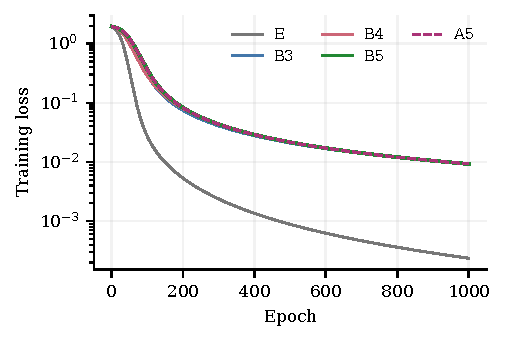
\includegraphics[width=.49\linewidth]{figures/fig_loss_revision_cora.pdf}
\caption{Complete 1000-epoch Cora/GCN training-loss trajectories, with a logarithmic loss axis. Scores are tabulated in Table~\ref{tab:revision-cora}; test data do not select these curves or their run length.}
\label{fig:loss-cora}
\end{figure}

B5 final test accuracy is 0.772 versus 0.771 for B3, and A5 equals B5 at the reported precision. The Euclidean head reaches 0.778. This is a near-tie among the manifold variants, not evidence of a robust graph-family win or an independent transport benefit. Recorded training times are descriptive and include concurrently running jobs; they are not controlled speed benchmarks. The full trajectories and checkpoints remain available for validation-selected analysis.

The new implementation uses actual Lorentz point parameters with closed-form exponential updates and parallel transport. Curvature gradients differentiate through the point homothety, unlike a partial derivative at fixed ambient coordinates. Classification uses one manifold prototype per class; text uses deterministic hashed tokens with an MLP or a two-layer Transformer; graph models use GCN, GAT, or GraphSAGE; recommendation uses a four-factor product distance with MF or origin-chart LightGCN propagation; KG uses grouped product states with a distance or transported-translation score. Synthetic product factors partition the requested total intrinsic dimension. This last architecture differs from the historical independent-tree groups, and the two protocols are not pooled.

KG evaluation in the revision ranks both heads and tails against every entity, filters other known true triples, uses average ranks for ties, and evaluates fixed full splits. MovieLens and Amazon Books use chronological leave-last-two-out per user. Recommendation excludes observed training items from negative draws and evaluates all-item, user-macro Recall@20/NDCG@20 with observed items masked. Yelp2018 instead preserves its published multi-positive test split, with one seed-42 original training interaction per user held out for validation. All test positives for each user contribute to Recall and normalized DCG. Both Euclidean and Lorentz LightGCN variants use two propagation layers; their geometry differs, while the graph operator is retained in both. Reuters retains all labels and uses binary cross entropy with micro/macro F1. Continual-learning experiments train for 1000 total epochs across five ordered tasks and report task-boundary average accuracy and forgetting; Rotated MNIST uses angles $0,36,72,108,144$ degrees, while Split CIFAR-100 uses five disjoint blocks of 20 class labels. No replay buffer is added. These protocols are predeclared in the executable configuration rather than adjusted after test scores are observed.

Appendix~\ref{app:run-ledger} contains the generated completion ledger and current coverage counts; all 705 retained configurations are complete, while 188 deferred configurations are excluded from completion claims. Original WN18RR, FB15k-237, and MNIST data were recovered from the hpc project directory. Tiny-ImageNet and YAGO3-10 have been acquired separately. The deterministic Amazon Books 20K-user subset has also been acquired from the official 2018 five-core release. An existing compute environment ImageNet-100 cache has now been located and its manifest verified: 114129 training images, 12560 held-out training images for validation, and 5000 official validation images reserved as test. This is the cached \texttt{clane9/imagenet-100} version with shorter-side-160px source images, subsequently resized by the declared input transform; it must not be conflated with an original-resolution protocol. The manifest hash and data source are retained with the execution records. Its 18 formerly blocked configurations were made runnable before the budget amendment and are now explicitly deferred. The Yelp subset is instantiated as the Yelp2018 interaction benchmark released by the LightGCN authors \citep{he2020lightgcn}, rather than an unspecified raw-review subset. It contains 31668 users, 38048 items, 1205591 retained training interactions, 31668 validation interactions, and 324147 original test interactions. The source commit and file hashes are recorded; the original test split is unchanged. This explicitly named, non-chronological protocol resolved the twelve data-blocked configurations; their execution is now deferred under the same budget amendment.


\subsection{Complete paired graph comparisons}
Table~\ref{tab:revision-breadth} extends the graph comparison beyond Cora. The generated table contains every dataset--encoder pair for which both B3 and B5 have completed the same 1000-epoch protocol. It uses final test accuracy consistently; validation-selected test metrics are retained separately in the machine-readable evidence file. Positive, tied, and negative differences are all kept. A positive single-seed difference is descriptive evidence for that configuration, not a significance claim or a substitute for equal-budget hyperparameter tuning.

% WWW_REFERENCE_STYLE
\begin{table*}[t]
\centering
\footnotesize\setlength{\tabcolsep}{4.2pt}\renewcommand{\arraystretch}{1.12}
\caption{Completed graph comparisons on compute environment, seed 42, 1000 epochs. Final test accuracy (\%) is the common endpoint; $\Delta$ is B5 minus B3 in percentage points. Every dataset--encoder pair with both completed runs is shown, including ties and negative differences. E is an architecture control with a Euclidean linear head. Dashes mean a comparator has not finished.}
\label{tab:revision-breadth}
\begin{adjustbox}{max width=\linewidth}
\begin{tabular}{llrrrrr}
\toprule
Dataset & Encoder & E & B3 & B5 & A5 & $\Delta$ \\
\midrule
arxiv & gat & \textbf{68.42} & 62.33 & \cellcolor{oursbg}62.41 & 62.45 & +0.08 \\
arxiv & gcn & \textbf{67.66} & 61.34 & \cellcolor{oursbg}61.19 & 61.21 & -0.16 \\
arxiv & sage & \textbf{68.32} & 63.39 & \cellcolor{oursbg}63.67 & 63.50 & +0.28 \\
citeseer & gat & \textbf{65.80} & 64.70 & \cellcolor{oursbg}64.60 & 64.60 & -0.10 \\
citeseer & gcn & 63.70 & \textbf{65.60} & \cellcolor{oursbg}\textbf{65.60} & \textbf{65.60} & +0.00 \\
citeseer & sage & 62.30 & 66.50 & \cellcolor{oursbg}\textbf{66.60} & \textbf{66.60} & +0.10 \\
cora & gat & 66.60 & \textbf{67.90} & \cellcolor{oursbg}67.70 & 67.70 & -0.20 \\
cora & gcn & \textbf{77.80} & 77.10 & \cellcolor{oursbg}77.20 & 77.20 & +0.10 \\
cora & sage & 77.80 & \textbf{78.10} & \cellcolor{oursbg}78.00 & 78.00 & -0.10 \\
pubmed & gat & 71.80 & \textbf{75.90} & \cellcolor{oursbg}\textbf{75.90} & \textbf{75.90} & +0.00 \\
pubmed & gcn & \textbf{76.50} & 75.90 & \cellcolor{oursbg}75.90 & 75.90 & +0.00 \\
pubmed & sage & 74.20 & 75.10 & \cellcolor{oursbg}\textbf{75.20} & \textbf{75.20} & +0.10 \\
\bottomrule
\end{tabular}
\end{adjustbox}
\end{table*}


\subsection{Long-horizon classification, ranking, and retention audit}
\label{app:long-horizon-audit}
We distinguish a complete method block from individual full-length runs. The 20 Newsgroups pooled-token block contains all eight registered methods. Its separate Transformer block has six registered methods; WN18RR translation, MovieLens-1M, and Rotated MNIST each have eight. WN18RR distance has six registered methods. These tables include only completed runs and state their coverage; missing controls are not assigned scores. Deferred methods are counted separately from unfinished retained controls. All records use seed 42 and the registered stopping length. Raw result and trajectory digests, selected validation epochs, and available per-run source digests are retained in \texttt{tables/revision\_long\_horizon\_evidence.json}. These are descriptive comparisons of registered configurations, not a claim that every run has an identical complete source snapshot.

\paragraph{Text classification and checkpoint selection.}
The registry name \texttt{mlp} denotes a pooled-token encoder: deterministic lowercase word hashing into 29999 nonpadding token IDs, truncation to 256 tokens, learned 128-dimensional token embeddings, masked mean pooling, and a 32-dimensional linear projection. The official 20 Newsgroups training split is divided into 10182 training and 1132 stratified validation documents with seed 42; all 7532 official test documents are retained. Headers, footers, and quotes are removed. The encoder uses AdamW with step $10^{-3}$; geometric prototypes use base step $0.1$, curvature step $0.001$, momentum $0.9$, and initial curvature 1. These are fixed configurations, not a hyperparameter search. Validation accuracy is checked every epoch; the first maximizing checkpoint is selected after the complete 1000-epoch run, and its test scores are distinguished from the final checkpoint. All eight selected epochs have been checked against the raw validation trajectories.

% WWW_REFERENCE_STYLE
\begin{table}[!htbp]
\centering
\caption{\textbf{Complete 20 Newsgroups classification block.} Eight methods, 1000 epochs each, seed 42. The registry labels the pooled-token encoder as \texttt{mlp}. The first maximum validation-accuracy checkpoint selects each method\textquotesingle s test result; epochs are one-based. All scores are percentages. Final accuracy is a separately labeled endpoint, not an alternative selection rule.}
\label{tab:revision-text-audit}
\footnotesize\setlength{\tabcolsep}{5pt}\renewcommand{\arraystretch}{1.12}
\begin{tabular}{lrrrrr}
\toprule
Method & Selected epoch & Val. acc.\ $\uparrow$ & Test acc.\ $\uparrow$ & Test macro-F1\ $\uparrow$ & Final acc.\ $\uparrow$ \\
\midrule
E & 427 & \textbf{71.113} & \textbf{61.471} & \textbf{60.750} & \textbf{61.418} \\
B2 & 179 & 68.463 & 57.554 & 56.291 & 56.678 \\
B3 & 179 & 68.728 & 57.820 & 56.552 & 56.745 \\
B4 & 183 & 68.286 & 57.754 & 56.494 & 56.121 \\
\rowcolor{oursbg}
B5 & 182 & 68.551 & 57.674 & 56.449 & 56.213 \\
A5 & 182 & 68.551 & 57.687 & 56.461 & 56.213 \\
B35 & 179 & 68.728 & 57.820 & 56.560 & 56.798 \\
Shared & 179 & 68.728 & 57.674 & 56.457 & 56.028 \\
\bottomrule
\end{tabular}
\end{table}


\paragraph{Separate Transformer comparison.}
The Transformer retains the same tokenization, data partitions, output dimension, prototype configuration, and validation selection. It adds learned positional embeddings and two Transformer encoder layers, each with hidden dimension 128, four attention heads, feed-forward dimension 256, and zero dropout, before masked mean pooling and projection. Table~\ref{tab:revision-transformer-audit} reports all four retained methods, including the B3--B5 pair. The two runs record identical hashes for the runner, geometry, and structured-task source modules. Their validation maxima occur at epochs 648 and 451, respectively (one-based). Selected test accuracy is $54.673\%$ for B3 and $52.987\%$ for B5, a B5 difference of $-1.686$ percentage points; selected macro-F1 is also lower for B5. Final accuracy preserves this ordering. The E and A5 controls finish at validation-selected test accuracies $55.709\%$ and $54.169\%$, respectively. Thus all four retained methods are complete, while B2 and B4 remain deferred. A different encoder on the same dataset is not an independent task family.

% WWW_REFERENCE_STYLE
\begin{table}[!htbp]
\centering
\caption{\textbf{20 Newsgroups Transformer: completed method endpoints.} Each listed method finishes 1000 epochs, seed 42. The first maximum validation-accuracy checkpoint selects its test result; epochs are one-based. 4/6 registered methods complete; 2 methods deferred by the budget amendment. Every completed method is retained. All scores are percentages; final accuracy is separately labeled. Bold compares only the displayed rows; B5 is shaded.}
\label{tab:revision-transformer-audit}
\footnotesize\setlength{\tabcolsep}{5pt}\renewcommand{\arraystretch}{1.12}
\begin{tabular}{lrrrrr}
\toprule
Method & Selected epoch & Val. acc.\ $\uparrow$ & Test acc.\ $\uparrow$ & Test macro-F1\ $\uparrow$ & Final acc.\ $\uparrow$ \\
\midrule
E & 960 & \textbf{65.724} & \textbf{55.709} & \textbf{55.006} & \textbf{55.616} \\
B3 & 648 & 63.428 & 54.673 & 53.539 & 54.408 \\
\rowcolor{oursbg}
B5 & 451 & 61.749 & 52.987 & 52.485 & 52.894 \\
A5 & 592 & 62.544 & 54.169 & 53.213 & 53.120 \\
\bottomrule
\end{tabular}
\end{table}


\paragraph{Primary endpoints in the other registered families.}
Tables~\ref{tab:revision-kg-audit}--\ref{tab:revision-retention-audit} report final endpoints rather than substituting the best observed test checkpoint. WN18RR translation B5 MRR is $0.10230$, versus $0.17225$ for E, $0.12598$ for B3, $0.12596$ for B35, and $0.10232$ for B4; B5 and A5 agree at the displayed precision. On MovieLens-1M, B5 Recall@20 is slightly higher than B3, but the primary NDCG@20 is lower ($2.1560\%$ versus $2.2072\%$); E reaches $4.2943\%$. On Rotated MNIST, all eight methods are complete. B5 mean accuracy is $43.432\%$, versus $43.388\%$ for B35 and $43.296\%$ for shared curvature: small increases of $0.044$ and $0.136$ percentage points. However, E, B3, and B2 reach $43.800\%$, $43.752\%$, and $44.340\%$, respectively. Shared curvature gives the highest last-task accuracy, $98.530\%$, versus $98.470\%$ for B5. A last-task score does not measure retention of earlier tasks. Accordingly, these observations do not establish an additional positive task family or an isolated transport benefit. All completed primary and secondary endpoints are shown, with each deferred method explicitly identified.

The completed shared-curvature WN18RR control has MRR $0.10200$. Grouped B5 improves this narrowly by $0.000295$ absolute MRR ($0.289\%$ relative), while remaining below both fixed-curvature controls; Hits@10 is slightly lower than shared curvature ($30.600\%$ versus $30.616\%$). This mixed profile does not establish a broad grouped-curvature gain. The MovieLens-1M A5 endpoint equals B5 exactly in both stored primary NDCG@20 ($0.02156021$) and secondary Recall@20 ($0.05546358$). Equality is an observed ranking-score result for this run, not a claim that the optimizer trajectories are identical. Primary endpoint choice, full run lengths, and the original configurations are unchanged.

% WWW_REFERENCE_STYLE
\begin{table}[!htbp]
\centering
\caption{\textbf{Available full-length endpoints.} WN18RR transported-translation model, 2000 epochs. All-entity filtered head-and-tail ranking at the final checkpoint. MRR is primary; Hits scores are percentages. 7/8 registered methods complete; all completed rows are shown. 1 method is deferred by the budget amendment. Bold compares only the displayed completed rows, including rounded ties; B5 is shaded. Seed 42, fixed starting configuration, no equal-budget hyperparameter search.}
\label{tab:revision-kg-audit}
\footnotesize\setlength{\tabcolsep}{5pt}\renewcommand{\arraystretch}{1.12}
\begin{tabular}{lrrrr}
\toprule
Method & MRR $\uparrow$ & Hits@1 (\%) $\uparrow$ & Hits@3 (\%) $\uparrow$ & Hits@10 (\%) $\uparrow$ \\
\midrule
E & \textbf{0.17225} & 0.271 & \textbf{30.568} & \textbf{45.246} \\
B3 & 0.12598 & \textbf{2.106} & 18.427 & 35.354 \\
B4 & 0.10232 & 1.133 & 15.077 & 30.632 \\
\rowcolor{oursbg}
B5 & 0.10230 & 1.133 & 15.061 & 30.600 \\
A5 & 0.10230 & 1.133 & 15.061 & 30.600 \\
B35 & 0.12596 & \textbf{2.106} & 18.427 & 35.354 \\
Shared & 0.10200 & 1.101 & 14.853 & 30.616 \\
\bottomrule
\end{tabular}
\end{table}

% WWW_REFERENCE_STYLE
\begin{table}[!htbp]
\centering
\caption{\textbf{Available full-length endpoints.} MovieLens-1M product-distance MF, 1000 epochs. Final all-item user-macro scores after chronological splitting and observed-item masking. NDCG@20 is primary; Recall@20 is secondary. Both are percentages. 5/8 registered methods complete; all completed rows are shown. 3 methods are deferred by the budget amendment. Bold compares only the displayed completed rows, including rounded ties; B5 is shaded. Seed 42, fixed starting configuration, no equal-budget hyperparameter search.}
\label{tab:revision-recommendation-audit}
\footnotesize\setlength{\tabcolsep}{5pt}\renewcommand{\arraystretch}{1.12}
\begin{tabular}{lrr}
\toprule
Method & NDCG@20 $\uparrow$ & Recall@20 $\uparrow$ \\
\midrule
E & \textbf{4.2943} & \textbf{11.5563} \\
B3 & 2.2072 & 5.4967 \\
\rowcolor{oursbg}
B5 & 2.1560 & 5.5464 \\
A5 & 2.1560 & 5.5464 \\
B35 & 2.2069 & 5.4967 \\
\bottomrule
\end{tabular}
\end{table}

% WWW_REFERENCE_STYLE
\begin{table}[!htbp]
\centering
\caption{\textbf{Available full-length endpoints.} Rotated MNIST, five ordered tasks and 1000 total epochs without replay. Mean accuracy across all five tasks is primary; forgetting averages the first four tasks, in percentage points. Last-task accuracy is secondary. All rows use the final checkpoint. 8/8 registered methods complete; all completed rows are shown. Bold compares only the displayed completed rows, including rounded ties; B5 is shaded. Seed 42, fixed starting configuration, no equal-budget hyperparameter search.}
\label{tab:revision-retention-audit}
\footnotesize\setlength{\tabcolsep}{5pt}\renewcommand{\arraystretch}{1.12}
\begin{tabular}{lrrr}
\toprule
Method & Mean acc. (\%) $\uparrow$ & Forgetting (pp) $\downarrow$ & Last-task acc. (\%) $\uparrow$ \\
\midrule
E & 43.800 & 68.267 & 98.380 \\
B2 & \textbf{44.340} & \textbf{67.520} & 98.350 \\
B3 & 43.752 & 68.320 & 98.390 \\
B4 & 42.804 & 69.535 & 98.390 \\
\rowcolor{oursbg}
B5 & 43.432 & 68.715 & 98.470 \\
A5 & 43.378 & 68.782 & 98.350 \\
B35 & 43.388 & 68.807 & 98.400 \\
Shared & 43.296 & 68.927 & \textbf{98.530} \\
\bottomrule
\end{tabular}
\end{table}

\FloatBarrier

\subsection{Budget amendment and retained comparisons}
\label{app:scope-amendment}
On November 4, 2026, the remaining execution budget was reduced after 691 of the 893 registered configurations had completed. The decision used the observed outcomes and compute costs and is therefore exploratory. Of the 202 unfinished configurations, 14 are retained and 188 deferred. Table~\ref{tab:scope-amendment} enumerates every retained unfinished comparison. It preserves ongoing controls, supplies three missing Euclidean anchors, and completes one unopened model block with all six original methods. No completed result is excluded; the registry, raw trajectories, and intermediate checkpoints remain available. The amendment is recorded in \texttt{experiments/revision/execution\_scope.json} and linked to each deferred record.

\begin{table}[!htbp]
\centering
\caption{Remaining execution budget at the amendment. Counts refer to unfinished configurations on November 4, not new trials or completed results. All retained runs keep their registered seed, splits, settings, and full training length.}
\label{tab:scope-amendment}
\footnotesize\setlength{\tabcolsep}{5pt}\renewcommand{\arraystretch}{1.12}
\begin{tabular}{llrr}
\toprule
Dataset and model & Retained unfinished methods & Runs & Epochs \\
\midrule
Rotated MNIST / MLP & B35, shared & 2 & 1000 \\
20 Newsgroups / Transformer & A5, E & 2 & 1000 \\
MovieLens-1M / MF & B35, E & 2 & 1000 \\
WN18RR / translation & B4, E & 2 & 2000 \\
WN18RR / distance & E, B2, B3, B4, B5, A5 & 6 & 2000 \\
\midrule
Total retained unfinished & & 14 & \\
Deferred, never started & & 187 & \\
Deferred, partially trained & CIFAR-100 / ResNet-18 / B5 & 1 & \\
\bottomrule
\end{tabular}
\end{table}

The interrupted CIFAR-100 run is not reported as a completed visual benchmark or a numerical failure. Its available checkpoints and loss log are preserved. The broad dataset--encoder expansion and other unstarted ablations are deferred for budget reasons. Within the amended blocks, the retained method counts are four of six for the Transformer, seven of eight for WN18RR translation, five of eight for MovieLens-1M, and all eight for Rotated MNIST. All 705 retained configurations have now completed, including all 14 runs retained by this amendment. The original 893 registrations are not relabeled as completed; the 188 deferred configurations remain separately identified.

\paragraph{Hierarchy-motivated distance comparison.}
The retained WN18RR distance block replaces transported translation by a relation-weighted product-distance score,
\begin{equation*}
s(h,r,t)=-\sum_{g=1}^{4}\bigl(1+\|v_{r,g}\|_{K_g}^{2}\bigr)
d_{K_g}(x_{h,g},x_{t,g})^2,
\qquad v_{r,g}=\operatorname{Log}_{o_{K_g}}(x_{r,g}).
\end{equation*}
It directly tests metric fitting on the same hierarchical graph, with the matched Euclidean architecture replacing each factor distance and relation norm by their Euclidean counterparts. All six originally registered methods are retained together, including the Euclidean, fixed-curvature, and no-transport controls; no hyperparameter or stopping rule is changed to pursue a favorable endpoint. The score is symmetric in its entity arguments, so it does not itself encode edge direction. This is a model-specific test within KG completion, not an additional task family. MRR remains the primary final-checkpoint endpoint under full filtered head-and-tail ranking, and the existing single-seed qualification remains in force. All six methods have now completed 2000 epochs. Table~\ref{tab:revision-kg-distance-audit} gives B5 MRR $0.13685$, compared with $0.15722$ for E, $0.14078$ for B2, $0.14077$ for B3, $0.13688$ for B4, and $0.13691$ for A5. B5 does not improve the primary endpoint over any of these controls. Its higher Hits@3 than B2 and B3 does not reverse the MRR or Hits@10 comparison. These final results do not establish an additional task-family advantage.

% WWW_REFERENCE_STYLE
\begin{table}[!htbp]
\centering
\caption{\textbf{Available full-length endpoints.} WN18RR relation-weighted distance model, 2000 epochs. All six registered methods are retained under the budget amendment. All-entity filtered head-and-tail ranking at the final checkpoint. MRR is primary; Hits scores are percentages. 6/6 registered methods complete; all completed rows are shown. Bold compares only the displayed completed rows, including rounded ties; B5 is shaded. Seed 42, fixed starting configuration, no equal-budget hyperparameter search.}
\label{tab:revision-kg-distance-audit}
\footnotesize\setlength{\tabcolsep}{5pt}\renewcommand{\arraystretch}{1.12}
\begin{tabular}{lrrrr}
\toprule
Method & MRR $\uparrow$ & Hits@1 (\%) $\uparrow$ & Hits@3 (\%) $\uparrow$ & Hits@10 (\%) $\uparrow$ \\
\midrule
E & \textbf{0.15722} & \textbf{0.000} & \textbf{30.089} & \textbf{38.449} \\
B2 & 0.14078 & \textbf{0.000} & 25.973 & 37.572 \\
B3 & 0.14077 & \textbf{0.000} & 25.973 & 37.556 \\
B4 & 0.13688 & \textbf{0.000} & 27.361 & 34.923 \\
\rowcolor{oursbg}
B5 & 0.13685 & \textbf{0.000} & 27.393 & 34.907 \\
A5 & 0.13691 & \textbf{0.000} & 27.393 & 34.907 \\
\bottomrule
\end{tabular}
\end{table}

\FloatBarrier


\subsection{Complete product-factor reconstruction grid}
\label{app:complete-product-grid}
The four tree constructions are binary, 4-ary, 8-ary, and variable-branching trees. Each uses the full Cartesian grid of three node counts and four total intrinsic dimensions stated in Table~\ref{tab:revision-synthetic-complete}. The Lorentz product has $\min(4,d)$ factors whose dimensions sum to $d$; every factor fits the same tree observations. Each update samples 65536 ordered node pairs, removes self-pairs, and minimizes mean squared relative-distance error. A separate generator fixed at seed 1042 draws up to 100000 evaluation pairs once, again removing self-pairs; final distortion is mean absolute relative-distance error on that fixed set. This is a reconstruction diagnostic: evaluation pairs are not withheld from the training-pair distribution. All methods finish 2000 updates. The Euclidean control uses SGD with momentum 0.9 and step 10; the manifold methods use base step 10, curvature step 0.001, and the common geometric safeguards. This is a fixed-configuration comparison, not a validation-selected tuning study. In particular, the B5--B3 contrast combines curvature adaptation and step normalization, while B5--A5 isolates the cross-curvature state map. The full table makes both contrasts and the Euclidean result inspectable.
% WWW_REFERENCE_STYLE
\begingroup
\footnotesize\setlength{\tabcolsep}{4.2pt}\renewcommand{\arraystretch}{1.12}
\begin{longtable}{lrrrrrrrrr}
\caption{Complete product-factor reconstruction grid. Final fixed-pair distortion (lower is better) after 2000 updates, seed 42. Bold indicates the best value at the displayed precision; B5 is shaded. The last column reports the B5 reduction relative to B3 in percent, calculated from unrounded records. All baselines, including the stronger Euclidean control, are retained.}\label{tab:revision-synthetic-all}\\
\toprule
Tree & $n$ & $d$ & E & B2 & B3 & B4 & B5 & A5 & Reduction (\%) \\
\midrule
\endfirsthead
\toprule
Tree & $n$ & $d$ & E & B2 & B3 & B4 & B5 & A5 & Reduction (\%) \\
\midrule
\endhead
\bottomrule
\endfoot
Binary & 1000 & 2 & \textbf{0.41637} & 0.72640 & 0.72635 & 0.72403 & \cellcolor{oursbg}0.72399 & 0.72400 & 0.3247 \\
Binary & 1000 & 5 & \textbf{0.32602} & 0.66094 & 0.66133 & 0.65903 & \cellcolor{oursbg}0.65943 & 0.65945 & 0.2874 \\
Binary & 1000 & 10 & \textbf{0.29453} & 0.63097 & 0.63134 & 0.62930 & \cellcolor{oursbg}0.62969 & 0.62970 & 0.2620 \\
Binary & 1000 & 20 & \textbf{0.27958} & 0.61316 & 0.61350 & 0.61161 & \cellcolor{oursbg}0.61197 & 0.61198 & 0.2505 \\
Binary & 5000 & 2 & \textbf{0.69453} & 0.95452 & 0.95471 & 0.95440 & \cellcolor{oursbg}0.95459 & 0.95459 & 0.0125 \\
Binary & 5000 & 5 & \textbf{0.65076} & 0.94672 & 0.94693 & 0.94662 & \cellcolor{oursbg}0.94683 & 0.94683 & 0.0099 \\
Binary & 5000 & 10 & \textbf{0.63689} & 0.94239 & 0.94261 & 0.94229 & \cellcolor{oursbg}0.94250 & 0.94250 & 0.0111 \\
Binary & 5000 & 20 & \textbf{0.62965} & 0.93826 & 0.93848 & 0.93814 & \cellcolor{oursbg}0.93836 & 0.93836 & 0.0127 \\
Binary & 10000 & 2 & \textbf{0.84620} & 0.98018 & 0.98026 & 0.98016 & \cellcolor{oursbg}0.98024 & 0.98024 & 0.0026 \\
Binary & 10000 & 5 & \textbf{0.82480} & 0.97607 & 0.97616 & 0.97605 & \cellcolor{oursbg}0.97614 & 0.97614 & 0.0022 \\
Binary & 10000 & 10 & \textbf{0.81708} & 0.97329 & 0.97338 & 0.97327 & \cellcolor{oursbg}0.97336 & 0.97336 & 0.0028 \\
Binary & 10000 & 20 & \textbf{0.81226} & 0.97009 & 0.97018 & 0.97005 & \cellcolor{oursbg}0.97014 & 0.97014 & 0.0036 \\
4-ary & 1000 & 2 & \textbf{0.36051} & 0.50908 & 0.50823 & 0.50512 & \cellcolor{oursbg}0.50421 & 0.50422 & 0.7910 \\
4-ary & 1000 & 5 & \textbf{0.23455} & 0.38139 & 0.38131 & 0.37882 & \cellcolor{oursbg}0.37876 & 0.37878 & 0.6707 \\
4-ary & 1000 & 10 & \textbf{0.18215} & 0.34137 & 0.34100 & 0.33942 & \cellcolor{oursbg}0.33906 & 0.33907 & 0.5688 \\
4-ary & 1000 & 20 & \textbf{0.15829} & 0.32290 & 0.32242 & 0.32127 & \cellcolor{oursbg}0.32080 & 0.32081 & 0.5012 \\
4-ary & 5000 & 2 & \textbf{0.44106} & 0.87753 & 0.87796 & 0.87673 & \cellcolor{oursbg}0.87717 & 0.87717 & 0.0901 \\
4-ary & 5000 & 5 & \textbf{0.34468} & 0.85667 & 0.85718 & 0.85606 & \cellcolor{oursbg}0.85657 & 0.85657 & 0.0713 \\
4-ary & 5000 & 10 & \textbf{0.31659} & 0.84622 & 0.84675 & 0.84557 & \cellcolor{oursbg}0.84611 & 0.84611 & 0.0761 \\
4-ary & 5000 & 20 & \textbf{0.30328} & 0.83768 & 0.83823 & 0.83698 & \cellcolor{oursbg}0.83754 & 0.83754 & 0.0828 \\
4-ary & 10000 & 2 & \textbf{0.62564} & 0.94424 & 0.94446 & 0.94405 & \cellcolor{oursbg}0.94427 & 0.94427 & 0.0195 \\
4-ary & 10000 & 5 & \textbf{0.57078} & 0.93405 & 0.93430 & 0.93390 & \cellcolor{oursbg}0.93415 & 0.93415 & 0.0159 \\
4-ary & 10000 & 10 & \textbf{0.55361} & 0.92822 & 0.92847 & 0.92805 & \cellcolor{oursbg}0.92830 & 0.92831 & 0.0183 \\
4-ary & 10000 & 20 & \textbf{0.54395} & 0.92227 & 0.92253 & 0.92207 & \cellcolor{oursbg}0.92233 & 0.92233 & 0.0218 \\
8-ary & 1000 & 2 & \textbf{0.34629} & 0.39497 & 0.39423 & 0.39353 & \cellcolor{oursbg}0.39280 & 0.39281 & 0.3624 \\
8-ary & 1000 & 5 & \textbf{0.18629} & 0.24986 & 0.24962 & 0.24934 & \cellcolor{oursbg}0.24911 & 0.24912 & 0.2061 \\
8-ary & 1000 & 10 & \textbf{0.12706} & 0.21326 & 0.21275 & 0.21273 & \cellcolor{oursbg}0.21224 & 0.21225 & 0.2371 \\
8-ary & 1000 & 20 & \textbf{0.09254} & 0.19817 & 0.19757 & 0.19764 & \cellcolor{oursbg}0.19706 & 0.19706 & 0.2576 \\
8-ary & 5000 & 2 & \textbf{0.36754} & 0.78506 & 0.78563 & 0.78287 & \cellcolor{oursbg}0.78345 & 0.78346 & 0.2768 \\
8-ary & 5000 & 5 & \textbf{0.23428} & 0.74700 & 0.74772 & 0.74530 & \cellcolor{oursbg}0.74603 & 0.74605 & 0.2255 \\
8-ary & 5000 & 10 & \textbf{0.19336} & 0.72832 & 0.72909 & 0.72659 & \cellcolor{oursbg}0.72737 & 0.72738 & 0.2360 \\
8-ary & 5000 & 20 & \textbf{0.17304} & 0.71503 & 0.71583 & 0.71324 & \cellcolor{oursbg}0.71405 & 0.71406 & 0.2498 \\
8-ary & 10000 & 2 & \textbf{0.46059} & 0.89895 & 0.89931 & 0.89837 & \cellcolor{oursbg}0.89874 & 0.89874 & 0.0634 \\
8-ary & 10000 & 5 & \textbf{0.37142} & 0.88138 & 0.88180 & 0.88093 & \cellcolor{oursbg}0.88135 & 0.88135 & 0.0509 \\
8-ary & 10000 & 10 & \textbf{0.34542} & 0.87208 & 0.87252 & 0.87159 & \cellcolor{oursbg}0.87203 & 0.87203 & 0.0565 \\
8-ary & 10000 & 20 & \textbf{0.33156} & 0.86344 & 0.86388 & 0.86288 & \cellcolor{oursbg}0.86333 & 0.86333 & 0.0646 \\
Variable & 1000 & 2 & \textbf{0.37559} & 0.56828 & 0.56758 & 0.56467 & \cellcolor{oursbg}0.56395 & 0.56396 & 0.6402 \\
Variable & 1000 & 5 & \textbf{0.24945} & 0.45533 & 0.45542 & 0.45274 & \cellcolor{oursbg}0.45283 & 0.45285 & 0.5673 \\
Variable & 1000 & 10 & \textbf{0.21387} & 0.41568 & 0.41553 & 0.41362 & \cellcolor{oursbg}0.41348 & 0.41350 & 0.4926 \\
Variable & 1000 & 20 & \textbf{0.19139} & 0.39677 & 0.39651 & 0.39501 & \cellcolor{oursbg}0.39476 & 0.39477 & 0.4425 \\
Variable & 5000 & 2 & \textbf{0.51448} & 0.90613 & 0.90648 & 0.90565 & \cellcolor{oursbg}0.90600 & 0.90600 & 0.0529 \\
Variable & 5000 & 5 & \textbf{0.43579} & 0.89022 & 0.89062 & 0.88984 & \cellcolor{oursbg}0.89025 & 0.89025 & 0.0416 \\
Variable & 5000 & 10 & \textbf{0.41323} & 0.88205 & 0.88248 & 0.88165 & \cellcolor{oursbg}0.88208 & 0.88208 & 0.0449 \\
Variable & 5000 & 20 & \textbf{0.40134} & 0.87510 & 0.87553 & 0.87466 & \cellcolor{oursbg}0.87510 & 0.87510 & 0.0496 \\
Variable & 10000 & 2 & \textbf{0.68836} & 0.95593 & 0.95611 & 0.95582 & \cellcolor{oursbg}0.95599 & 0.95599 & 0.0123 \\
Variable & 10000 & 5 & \textbf{0.64379} & 0.94772 & 0.94792 & 0.94763 & \cellcolor{oursbg}0.94782 & 0.94782 & 0.0101 \\
Variable & 10000 & 10 & \textbf{0.62919} & 0.94285 & 0.94305 & 0.94273 & \cellcolor{oursbg}0.94294 & 0.94294 & 0.0118 \\
Variable & 10000 & 20 & \textbf{0.62107} & 0.93769 & 0.93790 & 0.93755 & \cellcolor{oursbg}0.93776 & 0.93776 & 0.0144 \\
\end{longtable}
\endgroup


\subsection{All long-horizon mechanism conditions}
% WWW_REFERENCE_STYLE
\begin{table*}[t]
\centering
\footnotesize\setlength{\tabcolsep}{4.2pt}\renewcommand{\arraystretch}{1.12}
\caption{Long-horizon hierarchy mechanism tests: final held-out pair distortion after 2000 updates (lower is better). All methods use seed 42 and identical pair splits. Only cases with completed B5, B3, and A5 are included. The best-fixed column requires all five B35 curvature settings and selects using final validation distortion, never test distortion. Missing comparisons remain dashes. These controlled synthetic cases are not additional real-data task families.}
\label{tab:revision-mechanism}
\begin{adjustbox}{max width=\linewidth}
\begin{tabular}{lrrrrrr}
\toprule
Case & B3 & B5 & A5 & Shared & B4 & Best fixed \\
\midrule
abrupt8 & 0.7417 & \cellcolor{oursbg}0.6176 & 0.6176 & 0.6143 & 0.5914 & \textbf{0.1637} \\
heterogeneous & 0.2510 & \cellcolor{oursbg}0.2470 & 0.2463 & 0.2543 & 0.2415 & \textbf{0.2182} \\
smooth2 & 0.3328 & \cellcolor{oursbg}0.3295 & 0.3296 & 0.3260 & 0.3202 & \textbf{0.1823} \\
smooth5 & 0.6225 & \cellcolor{oursbg}0.4347 & 0.4347 & 0.4479 & 0.4262 & \textbf{0.2058} \\
smooth8 & 0.7411 & \cellcolor{oursbg}0.4813 & 0.4813 & 0.5078 & 0.4719 & \textbf{0.2757} \\
static & 0.2734 & \cellcolor{oursbg}0.2727 & 0.2726 & 0.2785 & 0.2604 & \textbf{0.2011} \\
\bottomrule
\end{tabular}
\end{adjustbox}
\end{table*}

% WWW_REFERENCE_STYLE
\begin{table*}[t]
\centering
\footnotesize\setlength{\tabcolsep}{4.2pt}\renewcommand{\arraystretch}{1.12}
\caption{Matched five-initialization comparison, 2000 updates per run. B35, B5, and A5 each use $K_0\in\{0.03,0.1,0.3,1,3\}$, with configurations selected by final validation distortion. Test distortion is reported after selection. A case appears only when all 15 runs finish. The last column compares B5 with A5 at B5\textquotesingle s selected initialization, retaining the clean transport contrast.}
\label{tab:revision-selected-mechanism}
\begin{adjustbox}{max width=\linewidth}
\begin{tabular}{lrrrrr}
\toprule
Case & Best fixed & B5 & Best A5 & B5 $K_0$ & Matched A5 \\
\midrule
abrupt8 & \textbf{0.1637} & \cellcolor{oursbg}0.1655 & 0.1663 & 0.03 & 0.1663 \\
heterogeneous & 0.2182 & \cellcolor{oursbg}0.2177 & \textbf{0.2174} & 0.1 & \textbf{0.2174} \\
smooth2 & 0.1823 & \cellcolor{oursbg}\textbf{0.1762} & 0.1763 & 0.1 & 0.1763 \\
smooth5 & \textbf{0.2058} & \cellcolor{oursbg}\textbf{0.2058} & 0.2061 & 0.03 & 0.2061 \\
smooth8 & 0.2757 & \cellcolor{oursbg}\textbf{0.2619} & 0.2624 & 0.03 & 0.2624 \\
static & 0.2011 & \cellcolor{oursbg}0.1952 & \textbf{0.1951} & 0.1 & \textbf{0.1951} \\
\bottomrule
\end{tabular}
\end{adjustbox}
\end{table*}


\subsection{New real-data protocols and complete comparisons}
The WordNet tasks use the full mammal and vehicle descendant subtrees in WordNet 3.0, including instances, and all internal transitive hypernym relations. The subtrees contain 1182 and 528 synsets, with 6542 and 2311 directed positive pairs, respectively. This is a custom missing-relation protocol and differs from the filtered mammals reconstruction benchmark of \citet{nickel2017poincare}. The corpus is accessed through NLTK \citep{nltkwordnet}. Ten percent of relations are reserved for validation and ten percent for test; the training split retains at least one incident relation for every nonisolated vertex. Filtered macro query MAP ranks every other synset and masks known positives outside the target split. The score penalizes both product distance and a reversed descendant--ancestor radial order.

Cora and Citeseer links use the Planetoid graphs \citep{planetoiddata}, with node identities but no attributes or class labels. Undirected pairs are canonicalized before splitting. Positive and negative pairs are disjoint across train, validation, and test, including reverse-edge equivalence; known positives are excluded from negative draws. The splits contain 5278 and 4552 positive pairs, respectively, with a matched number of negatives and an approximately 80/10/10 positive split that preserves training vertex coverage. Balanced-pair AP is primary and ROC-AUC is secondary; these scores do not estimate precision at the natural all-pairs prevalence.

Optical digits uses the 1797-image dataset distributed by scikit-learn \citep{sklearndigits}, with stratified training/validation/test counts 1078/359/360. Scaling is fit only on training observations. The 20 Newsgroups retrieval task \citep{sklearn20news} retains its official test set and partitions official training documents into 10182 training and 1132 validation queries, with 7532 test queries. Headers, footers, and quotes are removed. TF-IDF with at most 6000 features, a 128-component truncated SVD, and scaling are all fit exclusively on the training partition. A shared 128-unit tanh encoder produces eight features arranged as four two-dimensional factors; class proxies are optimized on their home manifolds. Retrieval uses observation embeddings, not class proxies, and the gallery contains training observations only. Primary same-class Recall@1 is the fraction of queries with a same-label top-ranked gallery item; secondary NDCG@10 uses same-class relevance. These are compact custom retrieval protocols rather than published leaderboard reproductions.

For each manifold method, the six configurations cross $K_0\in\{0.1,1,3\}$ with two base steps: $\{10,100\}$ for relation embeddings and $\{0.1,1\}$ for retrieval proxies. The Euclidean control receives the same two steps crossed with point-decay coefficients $\{0,10^{-4},10^{-2}\}$, also six runs. Other shared settings are $\beta=0.9$, $\rho=0.01$, $K\in[0.001,5]$, the canonical radius cap 4, the normalized trust cap 0.25, and the log-curvature cap 0.01. Auxiliary parameters use AdamW with learning rate $10^{-3}$ and decay $10^{-4}$. Temperature is restricted to $[e^{-3},e^3]$. Full-batch training spans all training examples each epoch. Validation loss is saved every epoch and the primary ranking metric every 25 epochs and at the final checkpoint. Final-checkpoint validation, not the best test score or best test epoch, selects the configuration. Training data, transformations, model capacity, and stopping length are identical across the relevant manifold comparisons. The canonical-radius constraint still makes physical-distance capacity curvature-dependent.

% WWW_REFERENCE_STYLE
Registered new-task completion counts: WordNet mammals: 30/30, Cora links: 30/30, Digits retrieval: 30/30, WordNet vehicles: 30/30, Citeseer links: 30/30, 20News retrieval: 30/30. Test comparison requires the full 30-run block.\par

% WWW_REFERENCE_STYLE
\begin{table*}[t]
\centering
\footnotesize\setlength{\tabcolsep}{4.2pt}\renewcommand{\arraystretch}{1.12}
\caption{Final-checkpoint test scores in percent; higher is better. Taxonomy: filtered query MAP; links: balanced-pair AP; retrieval: same-class Recall@1. Each method selects from six runs by final validation metric; all 30 configurations finish before any test evaluation. Matched A5 uses B5\textquotesingle s selected learning rate and initial curvature. Seed 42; 1000 epochs. Every completed task is retained, including ties and negative differences.}
\label{tab:new-tasks-all}
\begin{adjustbox}{max width=\linewidth}
\begin{tabular}{lrrrrrr}
\toprule
Task & E & B3 & B35 & B5 & A5 & Matched A5 \\
\midrule
WordNet mammals & 8.26 & 8.49 & 8.31 & \cellcolor{oursbg}8.29 & \textbf{8.96} & 8.38 \\
Cora links & \textbf{93.46} & \textbf{93.46} & \textbf{93.46} & \cellcolor{oursbg}\textbf{93.46} & \textbf{93.46} & \textbf{93.46} \\
Digits retrieval & 96.39 & 96.67 & 96.67 & \cellcolor{oursbg}\textbf{96.94} & \textbf{96.94} & \textbf{96.94} \\
WordNet vehicles & 8.42 & 8.40 & 7.80 & \cellcolor{oursbg}\textbf{8.50} & 8.27 & 8.27 \\
Citeseer links & 91.91 & 91.91 & \textbf{91.92} & \cellcolor{oursbg}\textbf{91.92} & \textbf{91.92} & \textbf{91.92} \\
20News retrieval & 42.31 & \textbf{43.49} & \textbf{43.49} & \cellcolor{oursbg}\textbf{43.49} & 43.45 & 43.45 \\
\bottomrule
\end{tabular}
\end{adjustbox}
\end{table*}


\FloatBarrier
\subsection{Recorded non-loss trajectory checkpoints}
\begin{table}[H]
\centering
\caption{\textbf{Historical KG metric checkpoints.} Recorded MRR, Hits@10 and learned curvature spread. Loss alone is plotted in Figure~\ref{fig:kg-loss}.}
\label{tab:kg-checkpoints}
\footnotesize\setlength{\tabcolsep}{4.2pt}\renewcommand{\arraystretch}{1.12}
\begin{adjustbox}{max width=\linewidth}
\begin{tabular}{lrrrrr}
\toprule
Epoch & B3 MRR & B4 MRR & B3 Hits@10 & B4 Hits@10 & B4 $K_{\rm std}$ \\
\midrule
100 & 0.1331 & 0.1334 & 0.3500 & 0.3500 & 0.0765 \\
300 & 0.1386 & 0.1361 & 0.3638 & 0.3688 & 0.2530 \\
500 & 0.1217 & 0.1250 & 0.3463 & 0.3575 & 0.2823 \\
800 & 0.1353 & 0.1384 & 0.3688 & 0.3750 & 0.2867 \\
1000 & 0.1356 & 0.1422 & 0.3588 & 0.3825 & 0.2886 \\
1500 & 0.1323 & 0.1321 & 0.3463 & 0.3538 & 0.2931 \\
1900 & 0.1337 & 0.1326 & 0.3337 & 0.3613 & 0.2946 \\
1999 & 0.1223 & 0.1355 & 0.3500 & 0.3563 & 0.2948 \\
\bottomrule
\end{tabular}
\end{adjustbox}
\end{table}

\begin{table}[H]
\centering
\caption{\textbf{Smooth-drift validation distortion and curvature states.} All methods start at $K_0=1$. $K_1,\ldots,K_4$ are B5 states. These are fixed checkpoints of the complete recorded trajectories, distinct from validation-selected initialization comparisons.}
\label{tab:drift-states}
\footnotesize\setlength{\tabcolsep}{4.2pt}\renewcommand{\arraystretch}{1.12}
\begin{adjustbox}{max width=\linewidth}
\begin{tabular}{lrrrrrrrr}
\toprule
Drift & Update & B3 & B5 & A5 & $K_1$ & $K_2$ & $K_3$ & $K_4$ \\
\midrule
2$\times$ & 1 & \textbf{0.9852} & \cellcolor{oursbg}\textbf{0.9852} & \textbf{0.9852} & 1.000 & 1.000 & 1.000 & 1.000 \\
2$\times$ & 100 & 0.3601 & \cellcolor{oursbg}\textbf{0.3568} & 0.3570 & 1.007 & 1.034 & 1.062 & 1.066 \\
2$\times$ & 500 & 0.3286 & \cellcolor{oursbg}0.3277 & \textbf{0.3276} & 0.978 & 1.052 & 1.082 & 1.096 \\
2$\times$ & 1000 & 0.3230 & \cellcolor{oursbg}0.3217 & \textbf{0.3216} & 0.909 & 1.035 & 1.104 & 1.127 \\
2$\times$ & 2000 & 0.3383 & \cellcolor{oursbg}0.3362 & \textbf{0.3361} & 0.743 & 0.879 & 1.019 & 1.119 \\
5$\times$ & 1 & \textbf{0.9852} & \cellcolor{oursbg}\textbf{0.9852} & \textbf{0.9852} & 1.000 & 1.000 & 1.000 & 1.000 \\
5$\times$ & 100 & 0.3440 & \cellcolor{oursbg}\textbf{0.3425} & \textbf{0.3425} & 1.004 & 1.026 & 1.054 & 1.064 \\
5$\times$ & 500 & \textbf{0.3506} & \cellcolor{oursbg}0.3529 & 0.3529 & 0.951 & 0.983 & 1.035 & 1.063 \\
5$\times$ & 1000 & 0.4660 & \cellcolor{oursbg}\textbf{0.4307} & \textbf{0.4307} & 0.836 & 0.793 & 0.812 & 0.834 \\
5$\times$ & 2000 & 0.6231 & \cellcolor{oursbg}\textbf{0.4382} & \textbf{0.4382} & 0.569 & 0.385 & 0.329 & 0.299 \\
8$\times$ & 1 & \textbf{0.9852} & \cellcolor{oursbg}\textbf{0.9852} & \textbf{0.9852} & 1.000 & 1.000 & 1.000 & 1.000 \\
8$\times$ & 100 & 0.3317 & \cellcolor{oursbg}0.3316 & \textbf{0.3314} & 1.001 & 1.019 & 1.044 & 1.061 \\
8$\times$ & 500 & 0.4446 & \cellcolor{oursbg}\textbf{0.4329} & \textbf{0.4329} & 0.929 & 0.912 & 0.932 & 0.958 \\
8$\times$ & 1000 & 0.5917 & \cellcolor{oursbg}\textbf{0.5123} & \textbf{0.5123} & 0.784 & 0.651 & 0.613 & 0.601 \\
8$\times$ & 2000 & 0.7411 & \cellcolor{oursbg}\textbf{0.4831} & \textbf{0.4831} & 0.444 & 0.223 & 0.165 & 0.138 \\
\bottomrule
\end{tabular}
\end{adjustbox}
\end{table}

